\documentclass[../main.tex]{subfiles}
\graphicspath{{\subfix{../images/}}}

\begin{document}

\chapter{Results}
% In Figure \ref{fig:executioncomparison} it's reported a graphical summary of the execution of one of the task implemented in the simulator: the figure compares the trajectory of the tooltip on the same task, recorded at the same repetition from a user in the assisted group and a user in the control group. With a color-coding applied on the trajectory that maps the distance error to a green-red-yellow color scale, the illustration shows how the assisted user was following the reference trajectory more closely than the unassisted. 

Figure \ref{fig:performancetraining} shows the performance trends for the four training tasks (\textit{Path, Rings, Pillars} and \textit{Exchange}), where the performance at each repetition is the average among the subjects in the assisted or control group. Apart from the \textit{Pillars} task, the trends are increasing both for the assisted group and the unassisted group. Most significantly, the performance in the assisted group is consistently higher than the one in the control group in all training tasks. 

\begin{figure}
    \centering
    \includegraphics[width=\textwidth]{images/performance_training.png}
    \caption{Performance Trend for the four Training Tasks. The value at each repetition is averaged across the subjects belonging to the same group. Error bars show the standard variation at each repetition}
    \label{fig:performancetraining}
\end{figure}

The standard deviation of the performance score is also displayed at each repetition with error bars that denote the range $\left[\mu - \frac{1}{2}\sigma; \mu + \frac{1}{2}\sigma\right]$, with $\mu$ and $\sigma$ the mean and standard deviation of the performance score, respectively. No significant difference is observed between the two groups and neither it is apparent a recognizable trend of deviation as a function of repetitions, \textit{i.e.} the error bars do not get wider nor narrower as the repetitions increase.

The gradual removal of haptic assistance that occurred daily during the training phase does not seem to have affected the performance of the subjects in the assisted group. All performance trends increase steadily from repetition 1 to repetition 12, without any significantly visible performance plateau. 

The performance on the four validation tasks (\textit{Thymectomy, Nephrectomy, Liver Resection} and \textit{Suturing}) recorded on the last day of the experimental phase is shown in Figure \ref{fig:performancevalidation} with boxplots. For each task, the graph reports the distribution of performances collected from the 4 subjects executing 3 repetitions. Crucially, neither the subjects in the assisted group nor the ones in the control group were guided with \acp{vf} on these tasks, nevertheless the performance recorded from the assisted subjects is distributed on higher values for all the tasks. 

\begin{figure}
    \centering
    \includegraphics[width=\textwidth]{images/performance_validation.png}
    \caption{Boxplots of the average performance of assisted subjects (blue) and unassisted subjects (orange) on the four validation tasks}
    \label{fig:performancevalidation}
\end{figure}

For both the assisted and unassisted groups, the performance is distributed on different values depending on the task, and so are the average values. This factor reflects how the tasks are different in terms of difficulty, and it is also reflected in the standard deviation of the performance. The standard deviation of distribution is, again, inconsistent when comparing the one calculated from group A and group C: in \textit{Thymectomy} and \textit{Nephrectomy} performance scores of assisted subjects are more spread out than the ones of unassisted subjects, while in \textit{Liver Resection} the variation is comparable and in \textit{Suturing} the performance of unassisted subjects has a higher deviation.
\begin{center}
    \begin{tabularx}{\linewidth}{||A|B|B|B||}
        \hline
\multicolumn{4}{||c||}{\textbf{Thymectomy}} \\
\hline\hline
& Mean & STD & Median \\
\hline
CONTROL & 0.38 & 0.01 & 0.37 \\
\hline
ASSISTED & 0.41 & 0.04 & 0.42 \\
\hline
\textbf{\% VAR} & \textbf{9.83\%} & \textbf{193.94\%} & \textbf{13.07\%} \\
\hline
% \label{tab:performance_Thymectomy}
\end{tabularx}
\end{center}
\begin{center}
    \begin{tabularx}{\linewidth}{||A|B|B|B||}
        \hline
        \multicolumn{4}{||c||}{\textbf{Nephrectomy}} \\
        \hline\hline
        & Mean & STD & Median \\
        \hline
        CONTROL & 0.68 & 0.06 & 0.71 \\
        \hline
        ASSISTED & 0.74 & 0.15 & 0.69 \\
        \hline
        \textbf{\% VAR} & \textbf{8.50\%} & \textbf{167.46\%} & \textbf{-2.71\%} \\
        \hline
        % \label{tab:performance_Nephrectomy}
    \end{tabularx}
\end{center}
\begin{center}
    \begin{tabularx}{\linewidth}{||A|B|B|B||}
        \hline
        \multicolumn{4}{||c||}{\textbf{LiverResection}} \\
        \hline\hline
        & Mean & STD & Median \\
        \hline
        CONTROL & 0.73 & 0.12 & 0.68 \\
        \hline
        ASSISTED & 0.90 & 0.15 & 0.83 \\
        \hline
        \textbf{\% VAR} & \textbf{23.42\%} & \textbf{28.85\%} & \textbf{21.54\%} \\
        \hline
% \label{tab:performance_LiverResection}
\end{tabularx}
\end{center}
\begin{center}
    \begin{tabularx}{\linewidth}{||A|B|B|B||}
        \hline
        \multicolumn{4}{||c||}{\textbf{Suturing}} \\
        \hline\hline
        & Mean & STD & Median \\
        \hline
        CONTROL & 0.84 & 0.05 & 0.85 \\
        \hline
        ASSISTED & 0.91 & 0.03 & 0.92 \\
        \hline
        \textbf{\% VAR} & \textbf{8.38\%} & \textbf{-25.39\%} & \textbf{8.44\%} \\
        \hline
        % \label{tab:performance_Suturing}
    \end{tabularx}
\end{center}

Quantitative results are reported in the tables above: for each task, the mean, standard deviation and median values of performance are compared between the assisted and the control group. Given the data scarcity and their non-Gaussian distribution, the most meaningful conclusions will be drawn from the median values. Apart from \textit{Nephrectomy} showing a slightly reduced median performance on assisted subject (accompanied, however, by a much larger standard deviation, as per Figure \ref{fig:performancevalidation}), all other tasks present an increase in the median performance, as high as $+21.54\%$. The variation in mean performance is, instead, always positive.

As a qualitative interpretation of the effect of virtual fixtures, Figure \ref{fig:executiontraining} and \ref{fig:executionevaluation} show, side by side, the trajectory of the \ee during the execution by an assisted subject and a non-assisted one. The trajectory is color-coded point-wise to reflect the distance error to the target trajectory, mesh or obstacle: although the figure does not recapitulate the general case, trajectories of unassisted subjects are visibly more erratic than the ones recorded from subjects in the assisted group. This is particularly evident for the training tasks (Figure \ref{fig:executiontraining}), where the haptic feedback force is acting to correct the teleoperation. The same qualitative interpretation, though, is valid for the evaluation tasks in Figure \ref{fig:executionevaluation}: however, if the tooltip's path seems more stable and less noisy in the execution of training tasks from assisted subjects, the same pattern of stability is not consistent. In this case, nevertheless, no assistance feedback force is applied to correct the execution.

\begin{figure}
    \centering
    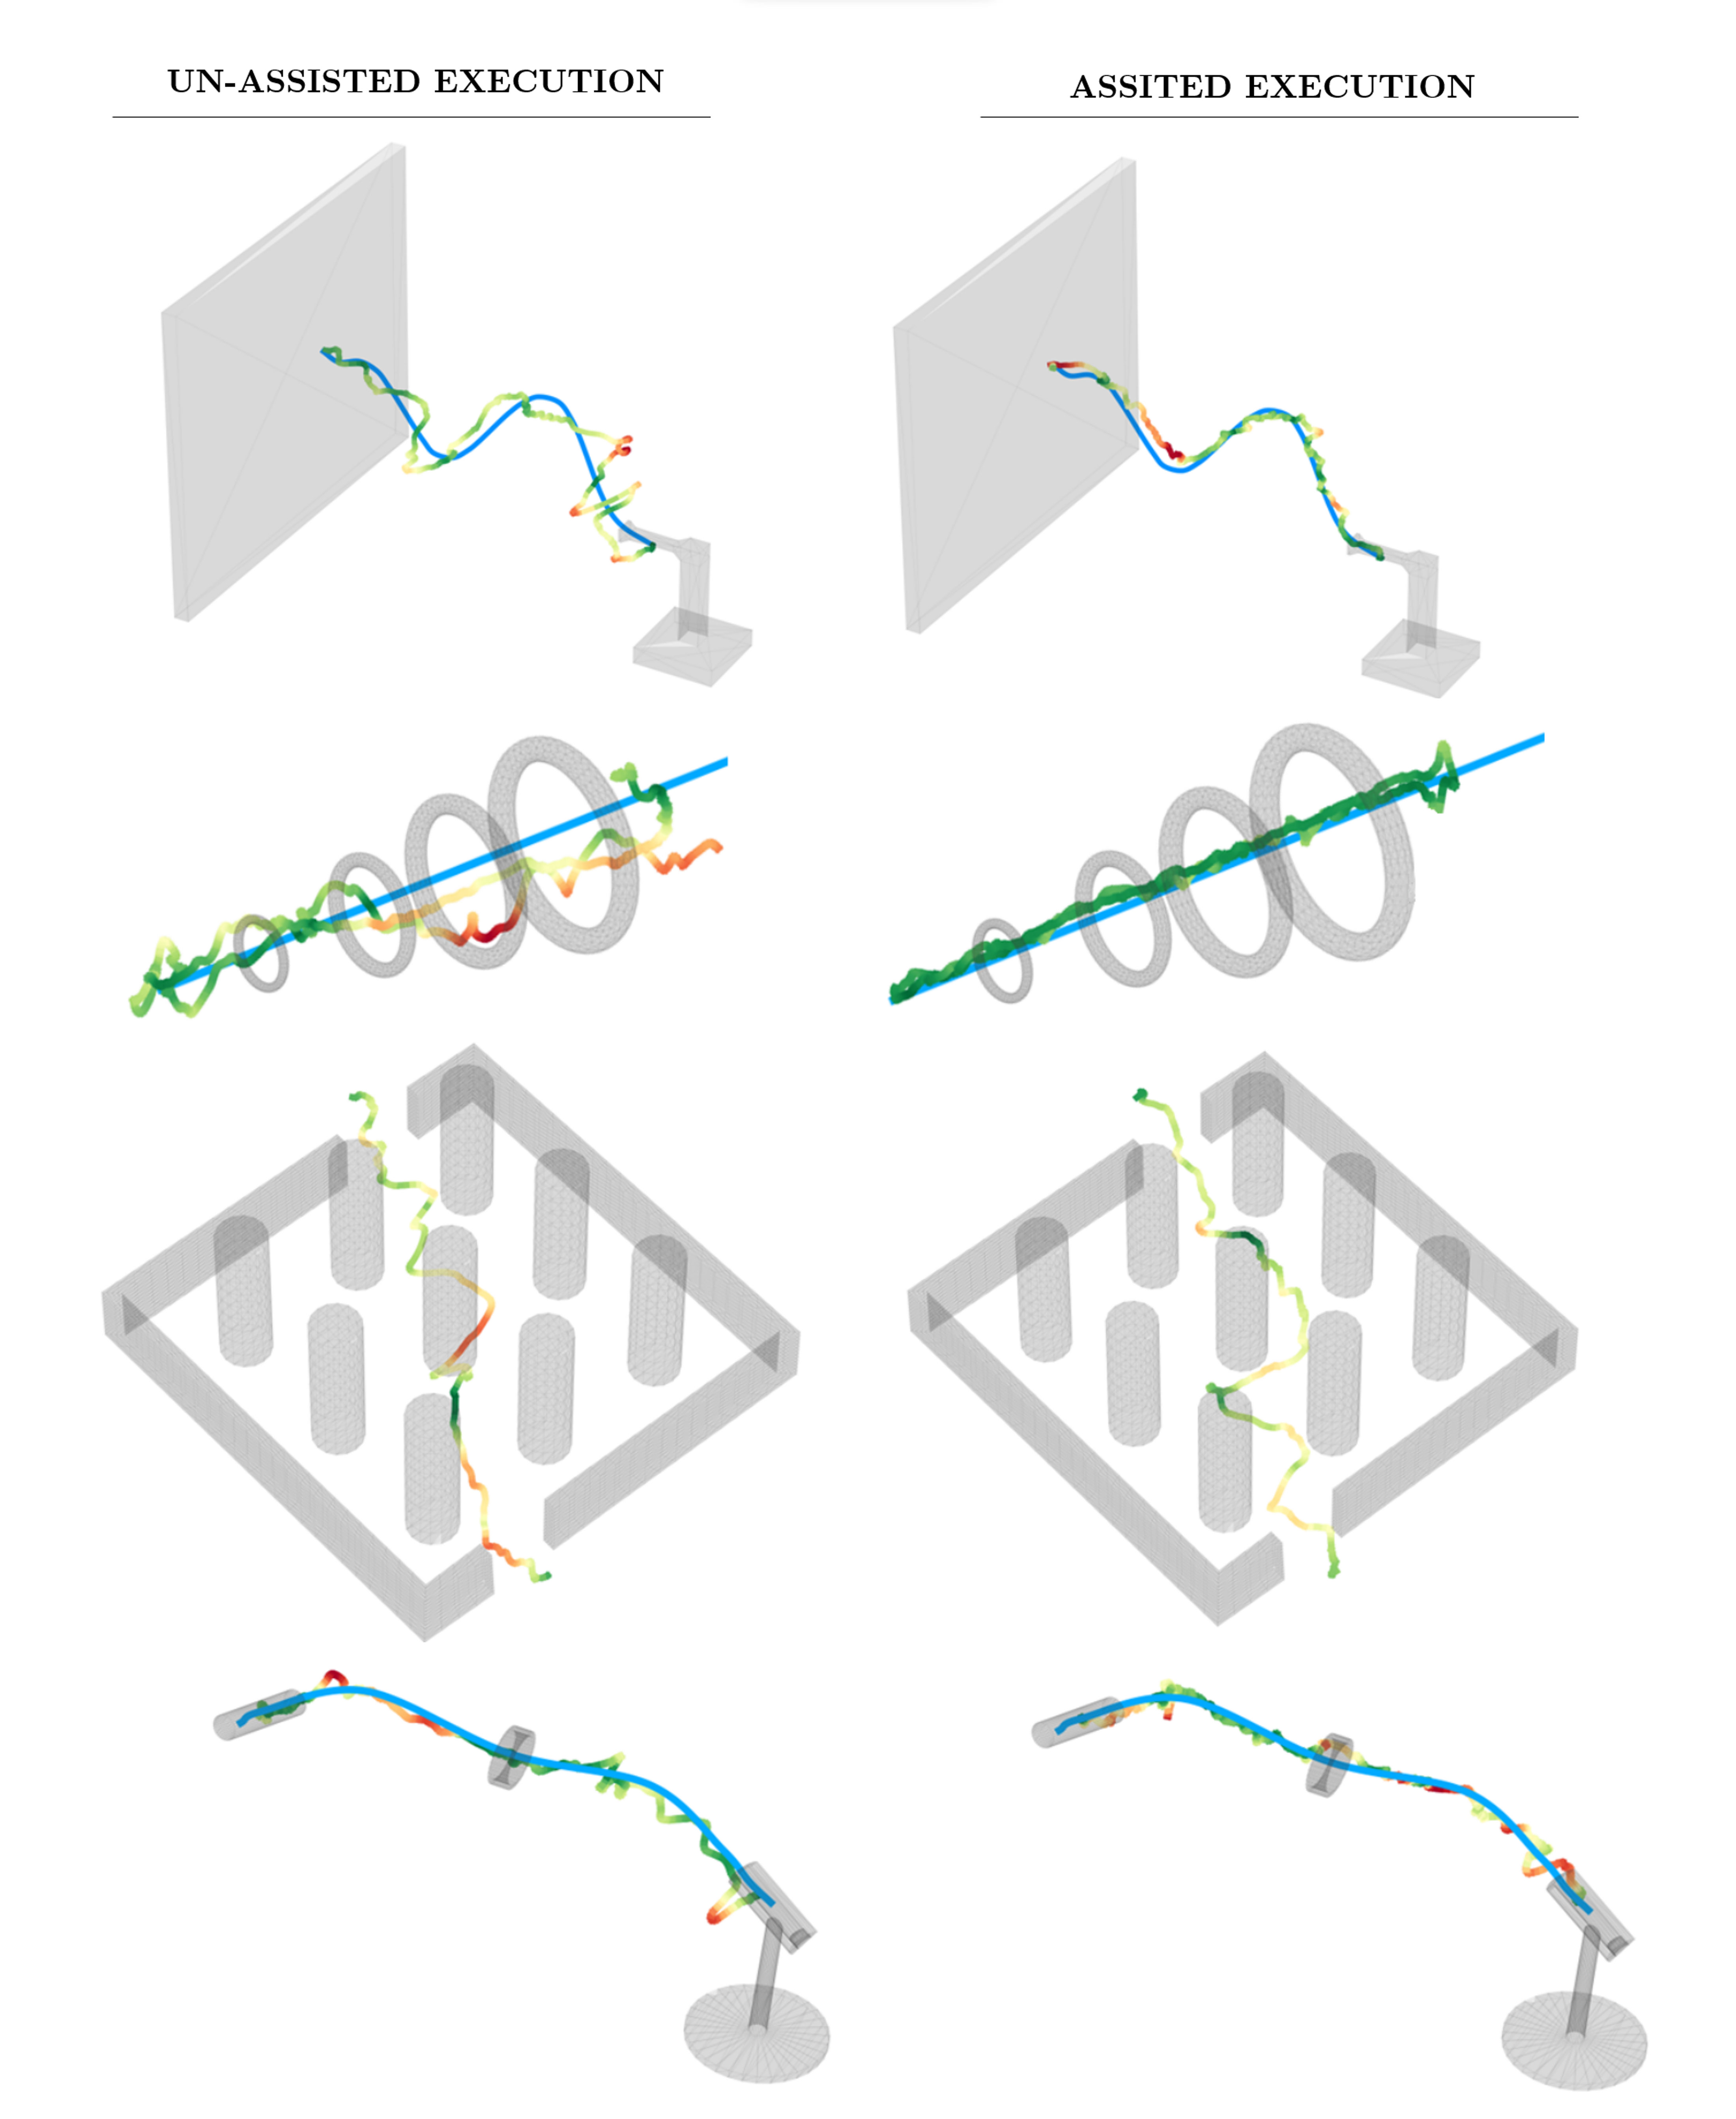
\includegraphics[width=\textwidth]{images/execution_training.png}
    \caption{Comparison in the execution of the 4 training tasks from a subject in the control group (left) and a subject in the assisted group (right). The End-Effector trajectory is color-coded according to the distance error from the target or obstacles. From top to bottom, the tasks are: \textit{Path}, \textit{Rings}, \textit{Pillars} and \textit{Exchange}.}
    \label{fig:executiontraining}
\end{figure}
\begin{figure}
    \centering
    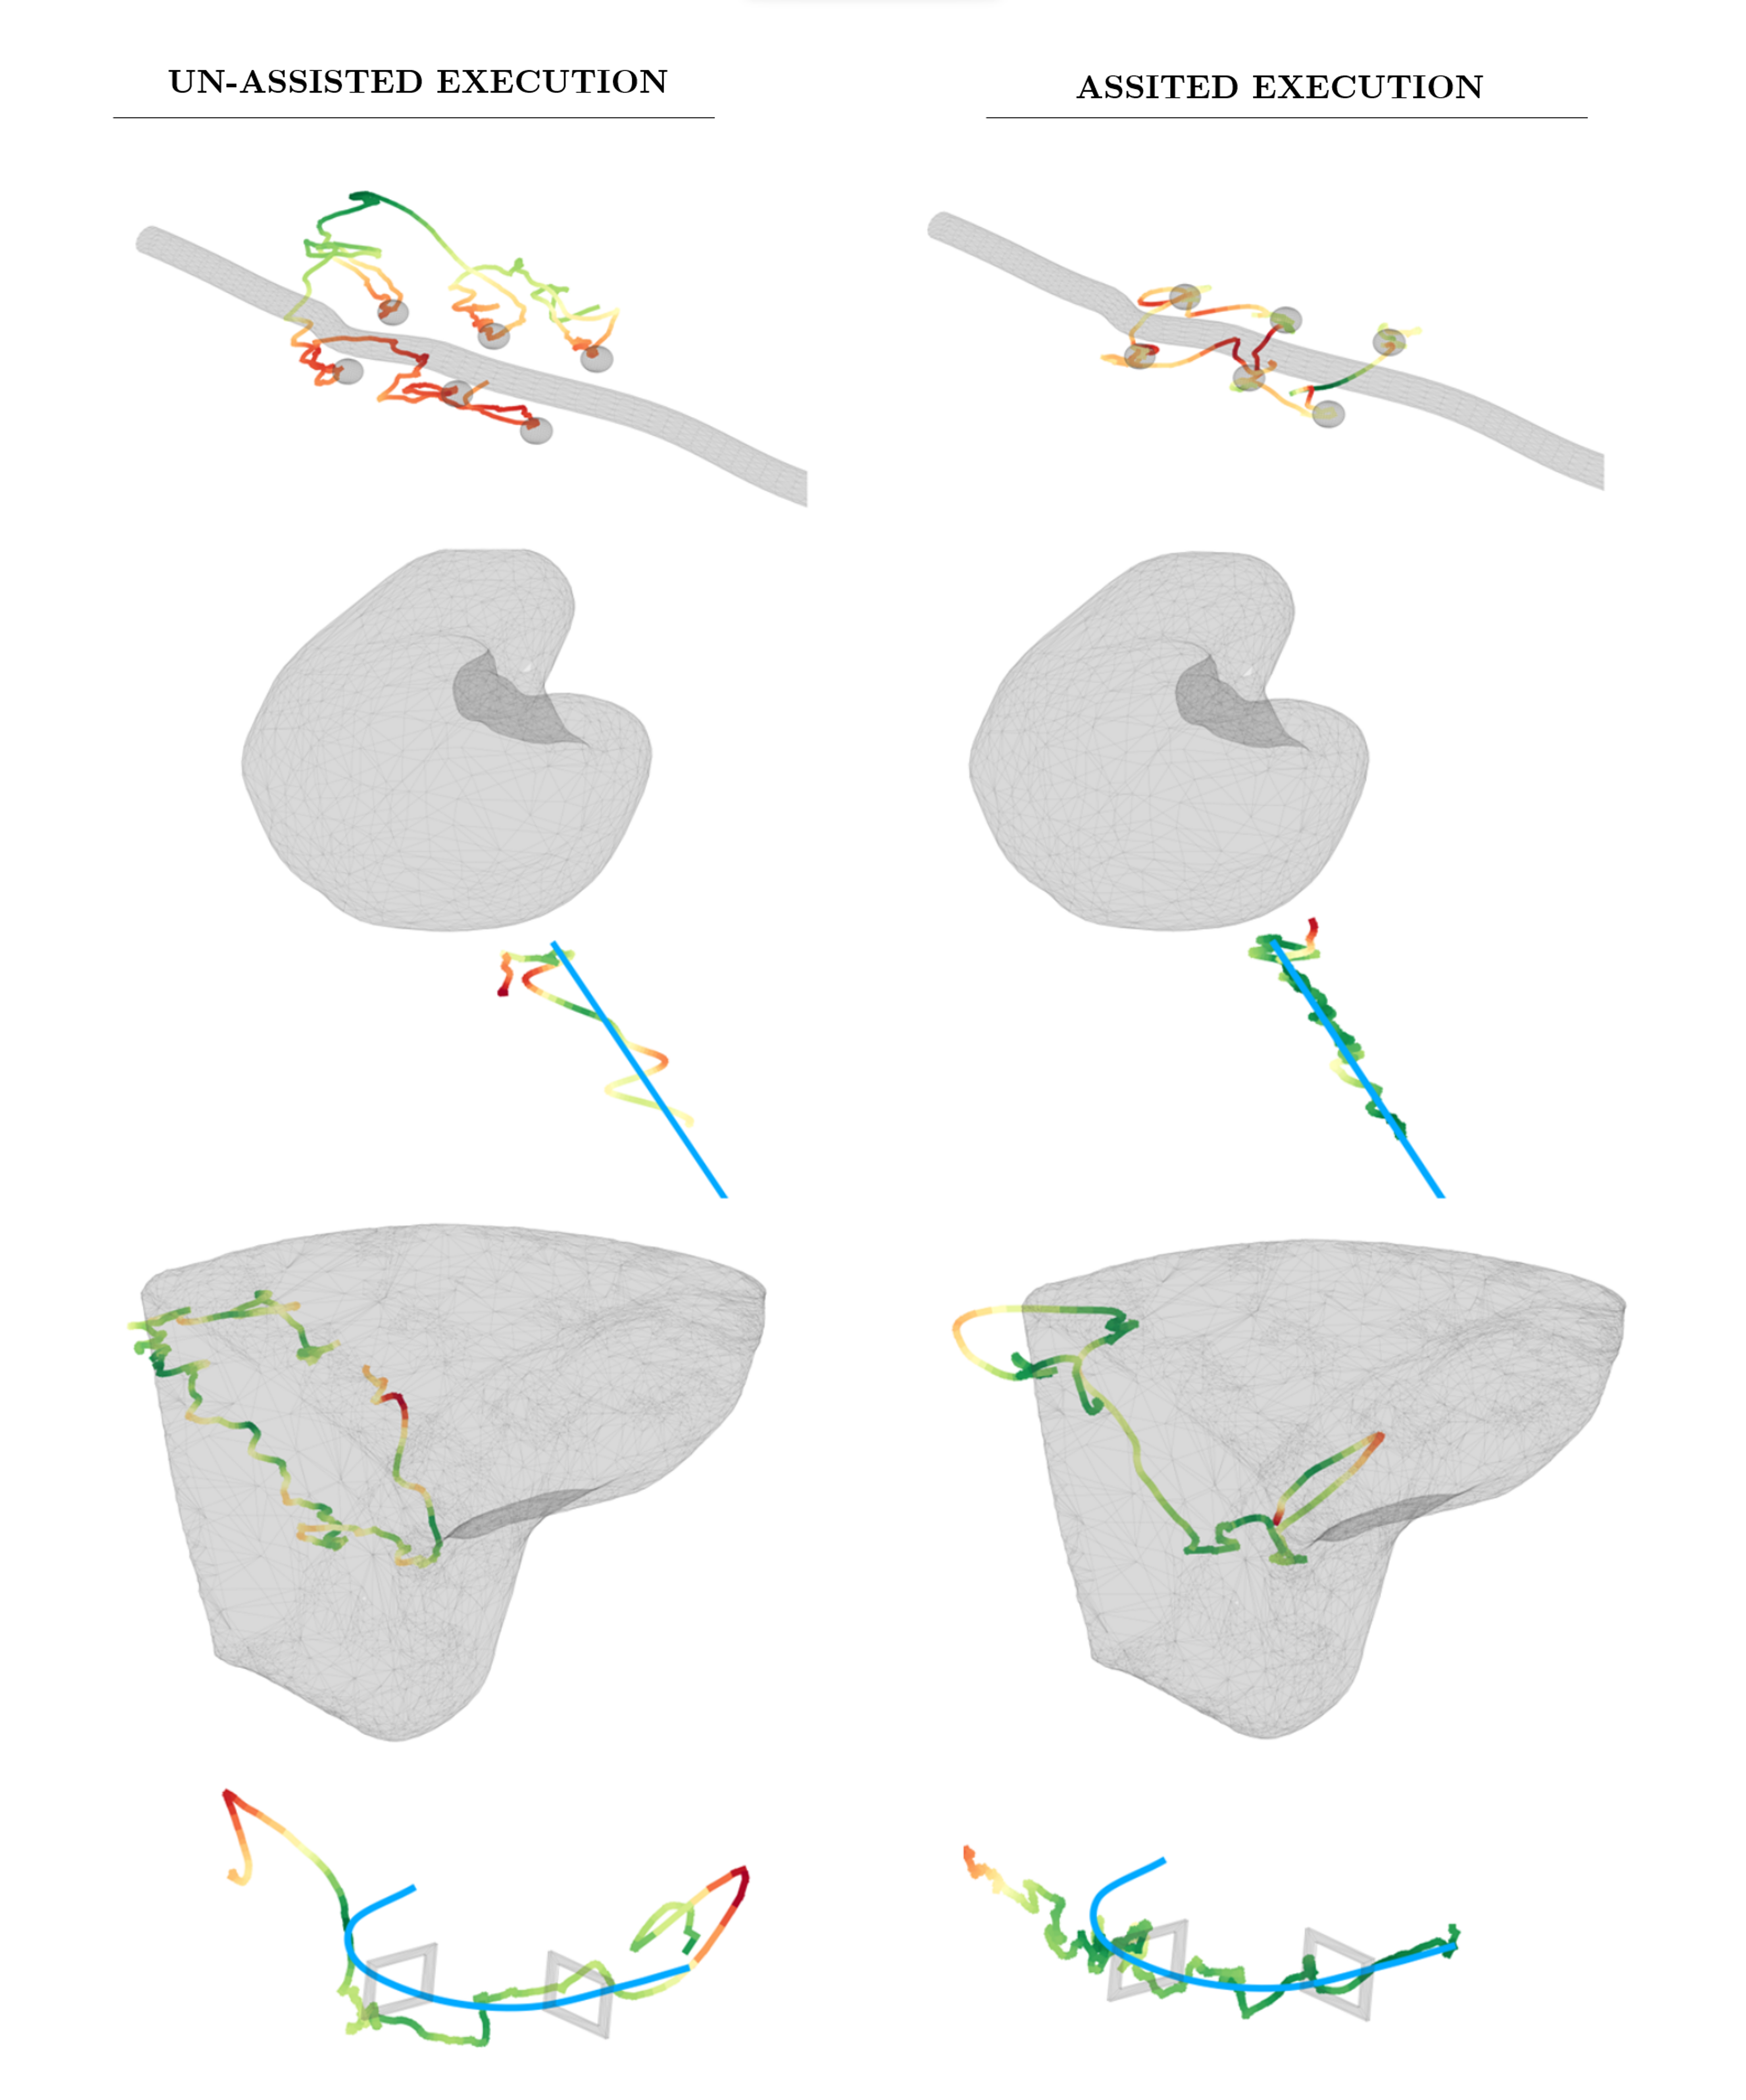
\includegraphics[width=\textwidth]{images/execution_evaluation.png}
    \caption{Comparison in the execution of the 4 evaluation tasks from a subject in the control group (left) and a subject in the assisted group (right). The End-Effector trajectory is color-coded according to the distance error from the target or obstacles. From top to bottom, the tasks are: \textit{Thymectomy, Nephrectomy, Liver Resection} and \textit{Suturing}.}
    \label{fig:executionevaluation}
\end{figure}

% BIBLIOGRAPHY
% \bibliographystyle{unsrt}
% \bibliography{refs.bib}

\end{document}